\chapter{Parasitic Files: ITF, the Mapping File, and SPEF}

\begin{tldr}
\begin{itemize}
  \item \textbf{Callback to Chapter 8 (CTS Spec):} Last chapter, the CTS spec told the tool how to build the clock. This chapter, parasitic files tell the tool (and the STA engine) what every wire it just built \emph{actually} does electrically.
  \item The \textbf{ITF} is the foundry's description of the metal stack: thicknesses, resistivities, dielectric constants. It is the source of truth for everything downstream.
  \item The \textbf{mapping file} bridges LEF/DEF layer names (\texttt{M3}, \texttt{VIA12}) to ITF layer indices. One typo here silently corrupts all RC.
  \item \textbf{SPEF} is the per net RC tree the extractor emits. Half of signoff timing debug is reading SPEF by hand.
\end{itemize}
\end{tldr}

\begin{hook}
The router placed an 80\,\textmu m wire on M3 between two flops. STA reports 47\,ps of delay on that net. Where did the 47 come from? Not from the cell. Not from the SDC. It came from a chain of files most engineers never open: a foundry ITF, a tiny mapping file, and a SPEF that the extractor cooked up at 3am during signoff. This chapter cracks that chain open.
\end{hook}

\section{ITF: The Interconnect Technology File}

The \textbf{ITF} (Interconnect Technology File) is a foundry deliverable that describes the back end of line stack exactly as the extraction engine sees it. Every metal layer has a thickness, a minimum width, a sheet resistance, and an etch profile. Every dielectric layer between metals has a thickness and a relative permittivity $\varepsilon_r$. Nothing in your timing comes out right if the ITF is wrong.

\begin{keyidea}
The ITF is not read by Innovus or PrimeTime directly. It is compiled by the foundry's extraction vendor (Synopsys StarRC, Cadence QRC) into a binary \textbf{TLU+} file or \textbf{QRC techfile}. That binary is what the extractor actually loads. The ITF is the human readable source; the TLU+ is the artifact your flow consumes.
\end{keyidea}

A small excerpt looks like this:

\begin{lstlisting}[style=eda,caption={ITF excerpt for a 7nm-ish stack.}]
TECHNOLOGY = my_7nm_stack
GLOBAL_TEMPERATURE = 25

CONDUCTOR M3 {
    THICKNESS    = 0.16
    WMIN         = 0.07
    SMIN         = 0.07
    RPSQ         = 0.072
    ETCH_VS_WIDTH { VALUES = (0.07, 0.005) (0.20, 0.008) }
}

DIELECTRIC ILD3 {
    THICKNESS = 0.20
    ER        = 2.7
}

DIELECTRIC ILD3_CAP {
    THICKNESS = 0.05
    ER        = 4.1   # nitride cap layer
}
\end{lstlisting}

Read it top down. M3 is 0.16\,\textmu m thick, the narrowest wire allowed is 70\,nm, the sheet resistance is 0.072\,$\Omega/\square$, and the etch shrinks the drawn width by a width dependent amount. Below M3 sits a 200\,nm ILD with $\varepsilon_r = 2.7$ (a low-k oxide), capped by a thin nitride layer at $\varepsilon_r = 4.1$. The extractor combines all of this with the actual routed geometry to produce R and C per segment.

\begin{hook}{The ITF is the stack's birth certificate}
The \textbf{foundry ships} an ITF that \textbf{freezes} the metal stack's electrical truth. Lose it, mis version it, or load the wrong corner, and \textbf{every SPEF downstream is fiction}.
\end{hook}

\begin{gut}
You see a TLU+ file in your flow but no ITF anywhere in the release. Is that normal? \gutans{Yes. Foundries often ship only the compiled TLU+ (and sometimes a redacted ITF) because the full ITF reveals proprietary process details. You consume the TLU+; you trust the foundry compiled it from the right ITF.}
\end{gut}

\section{The Mapping File: Tiny, Mission Critical}

The router speaks LEF/DEF layer names: \texttt{M1}, \texttt{M2}, \texttt{VIA12}. The ITF speaks its own layer indices and internal names. The \textbf{mapping file} (sometimes called the \texttt{nxtgrd} map, the \texttt{layer\_map}, or the \texttt{tech2itf} map) is the one line per layer dictionary that joins them.

\begin{lstlisting}[style=eda,caption={A tiny but mission critical mapping file.}]
# LEF/DEF name   ITF name      type
M1               METAL1        routing
M2               METAL2        routing
M3               METAL3        routing
VIA12            VIA1          via
VIA23            VIA2          via
\end{lstlisting}

If \texttt{M3} in the LEF is wrongly mapped to \texttt{METAL2} in the ITF, the extractor happily uses the thinner METAL2 thickness for every M3 segment in your design. Resistance is wrong by a constant factor. Capacitance is wrong by a different constant factor. Your STA looks clean. Silicon comes back broken.

\begin{pitfall}
A missing mapping line does \emph{not} always error out. Some flows fall back to a default layer or skip extraction on that layer entirely. You will see a warning buried in the extractor log and a SPEF that is missing parasitics on, say, every M7 net. Always grep the extraction log for \texttt{WARN} and \texttt{unmapped}.
\end{pitfall}

\section{SPEF: Where Parasitics Become a File You Read}

\textbf{SPEF} (Standard Parasitic Exchange Format) is the IEEE 1481 text format the extractor writes once per net. It contains the routed net's RC tree: every pin, every internal node (where a wire bends or branches), every R segment between nodes, and every C to ground (or coupling C to neighbor nets).

\move{1}{Set up the net.} Imagine a net \texttt{n42} driven by \texttt{U1/Y}, fanning out to two flop D pins, \texttt{FF1/D} and \texttt{FF2/D}. The router put down 80\,\textmu m of M3 total: 40\,\textmu m from the driver to a branch point, then 20\,\textmu m to each sink.

\move{2}{Compute the resistances.} M3 RPSQ is 0.072\,$\Omega/\square$. Wire width is 70\,nm, so squares per micron $= 1/0.07 \approx 14.3$. R per micron $= 14.3 \times 0.072 \approx 1.03\,\Omega/\text{\textmu m}$. So the 40\,\textmu m driver segment is $\sim 41\,\Omega$ and each 20\,\textmu m sink segment is $\sim 21\,\Omega$.

\move{3}{Compute the capacitances.} At 7nm M3 a sane total C is roughly 0.18\,fF/\textmu m (ground + coupling lumped). 40\,\textmu m $\to$ 7.2\,fF; 20\,\textmu m $\to$ 3.6\,fF. Split each segment's C into two lumps at its endpoints (the $\pi$ model the extractor uses).

\move{4}{Lay out the nodes.} Call them \texttt{1} (driver pin), \texttt{2} (branch), \texttt{3} (FF1/D), \texttt{4} (FF2/D). Caps lump at nodes 1, 2, 3, 4. Resistors sit between 1--2, 2--3, 2--4.

\move{5}{Pick the cap totals at each node.} Driver pin node 1 gets $\sim 3.6$\,fF from half of the driver segment. Branch node 2 gets the other half of the driver segment plus half of each sink segment: $3.6 + 1.8 + 1.8 = 7.2$\,fF. Sink nodes 3 and 4 each get the other half of their sink segment: $\sim 1.8$\,fF each, plus the pin cap of the receiving flop ($\sim 1.5$\,fF), total $\sim 3.3$\,fF.

\move{6}{Write it as SPEF.} See Listing~\ref{lst:spef-n42}.

\move{7}{Sanity check the totals.} Total wire C: $3.6 + 7.2 + 3.3 + 3.3 = 17.4$\,fF, close to the $0.18 \times 80 = 14.4$\,fF wire estimate plus $2 \times 1.5$\,fF pin caps. Total R from driver to FF1: $41 + 21 = 62\,\Omega$. Numbers feel right for 7nm M3.

\begin{lstlisting}[style=eda,caption={SPEF snippet for net \texttt{n42}. Reduced and slightly idealized.},label={lst:spef-n42}]
*SPEF "IEEE 1481-1999"
*DESIGN "duc_top"
*DATE "Mon May 26 14:02:11 2026"
*VENDOR "Cadence"
*PROGRAM "Quantus"
*VERSION "21.1"
*DESIGN_FLOW "PIN_CAP NONE" "FULL_CONNECTIVITY"
*DIVIDER /
*DELIMITER :
*BUS_DELIMITER [ ]
*T_UNIT 1 PS
*C_UNIT 1 FF
*R_UNIT 1 OHM
*L_UNIT 1 HENRY

*D_NET n42 17.4
*CONN
*I U1:Y O *L 0 *D BUFX4
*I FF1:D I *L 1.5 *D DFFX1
*I FF2:D I *L 1.5 *D DFFX1
*CAP
1 n42:1        3.6
2 n42:2        7.2
3 n42:3        3.3
4 n42:4        3.3
*RES
1 n42:1 n42:2  41.0
2 n42:2 n42:3  21.0
3 n42:2 n42:4  21.0
*END
\end{lstlisting}

\begin{figure}[h]
\centering
\begin{tikzpicture}[
  node distance=14mm,
  pin/.style={draw, fill=black!10, minimum size=6mm, font=\small},
  inode/.style={circle, draw, fill=white, inner sep=1pt, font=\scriptsize},
  capn/.style={font=\scriptsize, blue!60!black},
  res/.style={font=\scriptsize, red!60!black, midway, above}
]
  \node[pin] (d) {U1/Y};
  \node[inode, right=22mm of d] (n2) {2};
  \node[pin, above right=6mm and 22mm of n2] (s1) {FF1/D};
  \node[pin, below right=6mm and 22mm of n2] (s2) {FF2/D};

  \draw[thick] (d) -- node[res]{$R_{12}=41\,\Omega$} (n2);
  \draw[thick] (n2) -- node[res]{$R_{23}=21\,\Omega$} (s1);
  \draw[thick] (n2) -- node[res, below]{$R_{24}=21\,\Omega$} (s2);

  \draw[blue!60!black, thick] (d) -- ++(0,-9mm) node[capn, below]{$C_1=3.6$\,fF};
  \draw[blue!60!black, thick] (n2) -- ++(0,-9mm) node[capn, below]{$C_2=7.2$\,fF};
  \draw[blue!60!black, thick] (s1) -- ++(0,-9mm) node[capn, below]{$C_3=3.3$\,fF};
  \draw[blue!60!black, thick] (s2) -- ++(0,-9mm) node[capn, below]{$C_4=3.3$\,fF};
\end{tikzpicture}
\caption{RC tree for net \texttt{n42} reconstructed from the SPEF in Listing~\ref{lst:spef-n42}. Caps shown as lumps to ground; resistors between nodes.}
\label{fig:rc-tree}
\end{figure}

\begin{pausebox}
Before you read on, stare at Listing~\ref{lst:spef-n42} and Figure~\ref{fig:rc-tree} side by side. The \texttt{*CAP} section is just a list of (node, value) pairs. The \texttt{*RES} section is just (from, to, value). Once that clicks, SPEF stops being scary and becomes a circuit netlist you can sketch on paper in 60 seconds.
\end{pausebox}

\section{How STA Actually Uses SPEF}

The STA engine does \emph{not} simulate the RC tree as a SPICE deck (way too slow for millions of nets). It reduces the tree to an \textbf{effective capacitance} $C_{\text{eff}}$ seen by the driver and an \textbf{Elmore delay} (or higher order moment) to each sink. CCS and ECSM models then use $C_{\text{eff}}$ to pick the right driver waveform from the \texttt{.lib}.

The \textbf{Elmore delay} to a sink is the sum, over every resistor $R_i$ on the path from driver to sink, of $R_i$ times the total downstream capacitance hanging off $R_i$.

\begin{hook}{Elmore = R times all the C it sees downstream}
For each \textbf{resistor on the path}, \textbf{multiply it by every cap downstream} of it, \textbf{sum the products}. Skip a downstream branch and your delay is wrong by the branch's contribution.
\end{hook}

Worked example for the path \texttt{U1/Y} $\to$ \texttt{FF1/D} in Figure~\ref{fig:rc-tree}:

\begin{itemize}
  \item $R_{12} = 41\,\Omega$ sees everything downstream of node 2: $C_2 + C_3 + C_4 = 7.2 + 3.3 + 3.3 = 13.8$\,fF.
  \item $R_{23} = 21\,\Omega$ sees only $C_3 = 3.3$\,fF.
\end{itemize}

$$ t_{\text{Elmore}} = 41 \times 13.8 + 21 \times 3.3 = 565.8 + 69.3 = 635.1\,\Omega\cdot\text{fF} = 0.635\,\text{ps}.$$

That is the \emph{wire delay} contribution at sink FF1/D. The driver's intrinsic delay (from the \texttt{.lib}, evaluated at the effective load) is added on top. The 47\,ps from the chapter opener is mostly the driver, with a small contribution from this Elmore term. Now you know where it came from.

\begin{gut}
If the router rerouted node 2 farther from the driver, doubling $R_{12}$ to 82\,$\Omega$, what happens to FF1's Elmore delay? \gutans{The first term doubles: $82 \times 13.8 = 1131.6$. Total becomes $1131.6 + 69.3 = 1200.9\,\Omega\cdot\text{fF} \approx 1.2$\,ps. The shared resistor near the driver dominates because it sees the entire downstream capacitance.}
\end{gut}

\section{SPEF Flavors and Corners}

SPEF is not a single file. The extractor emits one SPEF \emph{per RC corner}, and modern signoff loads them all under MMMC. The standard set is:

\begin{itemize}
  \item \textbf{Cworst}: worst case coupling cap. Used for setup analysis when long wires hurt the most.
  \item \textbf{Cbest}: best case (lowest) cap. Used for hold analysis where fast nets cause race conditions.
  \item \textbf{RCworst}: worst R \emph{and} worst C. Pessimistic for setup on resistive paths.
  \item \textbf{RCbest}: best R and best C. Optimistic; hold analysis on long wires.
  \item \textbf{Typical}: nominal corner for sanity and reporting.
\end{itemize}

\begin{figure}[h]
\centering
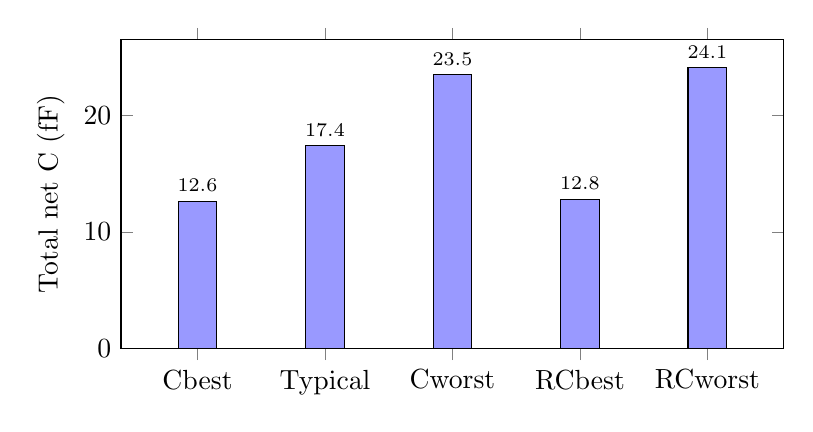
\begin{tikzpicture}
\begin{axis}[
  width=10cm, height=5.5cm,
  ybar, bar width=14pt,
  ylabel={Total net C (fF)},
  symbolic x coords={Cbest, Typical, Cworst, RCbest, RCworst},
  xtick=data, ymin=0,
  nodes near coords, nodes near coords style={font=\scriptsize},
  enlarge x limits=0.15,
]
\addplot[fill=blue!40] coordinates {
  (Cbest, 12.6) (Typical, 17.4) (Cworst, 23.5) (RCbest, 12.8) (RCworst, 24.1)
};
\end{axis}
\end{tikzpicture}
\caption{Extracted total C for net \texttt{n42} across the five RC corners. The same net, the same routing, five different SPEFs.}
\label{fig:corners}
\end{figure}

Five SPEFs per scenario. Multiply by your PVT corners, modes, and OCV settings, and the MMMC explosion from the back matter chapter stops being abstract: at Arm signoff you can easily be loading 40+ SPEFs in a single \texttt{create\_analysis\_view} grid.

\begin{pitfall}
Comparing the C of a net across two SPEFs and concluding "extraction is broken" is a classic rookie mistake. Check the header. If one is \texttt{*DESIGN\_FLOW "..."} Cworst and the other is Cbest, they are \emph{supposed} to differ by 30 to 50 percent. They are not the same file.
\end{pitfall}

\begin{sidebar}{DSPF vs SPEF vs SBPF}
\textbf{DSPF} (Detailed Standard Parasitic Format) is the older, Synopsys originated format. It preserves every internal node with explicit names like \texttt{n42:1234}, making it easy to map back to physical geometry. SPICE simulators love it. \textbf{SBPF} (Synopsys Binary Parasitic Format) is a compressed binary form for huge designs.

\textbf{SPEF} won as the lingua franca because IEEE standardized it, every vendor reads it, and it supports name mapping (\texttt{*NAME\_MAP}) to compress the file. Some analog teams still ship DSPF for block level SPICE sims, then the digital flow converts to SPEF for STA. At Arm you will mostly see SPEF; DSPF shows up only when a memory or analog macro hands you their extracted view.
\end{sidebar}

\begin{pdnote}{Why PD Cares about Parasitic Files}
\begin{itemize}
  \item \textbf{At Arm on Duc:} you will be staring at SPEF when a path mysteriously misses timing at signoff that was clean post route. Learning to grep \texttt{*D\_NET <netname>} out of a 4\,GB SPEF, sketch the RC tree, and hand compute Elmore is a core Innovus debugging skill. The first time a senior engineer asks "what's the Reff on the second branch?" you want to know exactly which lines to look at.
  \item \textbf{Generic PD engineer:} parasitic correlation between extractor outputs and silicon is one of the top three reasons a tapeout slips. If your team upgrades TLU+ mid project, every block's timing changes and you have to re-close. Understanding what an ITF, mapping file, and SPEF \emph{are} is the prerequisite to even having that conversation.
  \item \textbf{VLSI interview:} "Walk me through how a wire becomes a delay number in STA" is a standard question. The answer (geometry $\to$ ITF $\to$ TLU+ $\to$ extractor $\to$ SPEF $\to$ reduction $\to$ Elmore $\to$ .lib lookup) is what this chapter is about. Saying "the tool just figures it out" is a fast way to end the interview.
\end{itemize}
\end{pdnote}

\begin{checkpoint}
\mnemonic{ITF cooks the stack, the map joins the names, SPEF tells STA what the wire really is.}

You should now be able to:
\begin{itemize}
  \item Explain why the ITF lives upstream of TLU+ and never goes into Innovus directly.
  \item Read a five line mapping file and name what breaks if a line is missing.
  \item Sketch an RC tree from a \texttt{*D\_NET} block in a SPEF in under a minute.
  \item Compute Elmore delay to any sink given the tree.
  \item Name the five standard RC corners and which analysis each one feeds.
\end{itemize}
\end{checkpoint}
